
\documentclass{bioinfo}
\copyrightyear{2011}
\pubyear{2011}

\usepackage{comment}


\begin{document}
\firstpage{1}

\title{Correcting for bias in high throughput sequencing data}
\author[Jones \textit{et~al}]
{Daniel C. Jones\,$^{1,}$
\footnote{to whom correspondence should be addressed}\hspace{0.5em}
Walter L. Ruzzo\,$^{1,2}$
Xinxia Peng\,$^{3}$
Michael G. Katze$^{3}$
}

\history{Received on XXXXX; revised on XXXXX; accepted on XXXXX}

\address{
$^{1}$Deportment of Computer Science and Engineering, University of
Washington, Seattle, WA 98195-2350, USA\\
$^{2}$Fred Hutchinson Cancer Research Center, Seattle, WA 98109, USA\\
$^{3}$Department of Microbiology, University of Washington, Seattle, WA
98195-7242, USA}

\editor{Associate Editor: XXXXXXX}

\maketitle

\begin{abstract}

\section{Motivation:}

Quantification of sequence abundance in RNA-Seq and ChiP-Seq experiments is
often conflated with protocal-specific bias, influenced by PCR amplification,
and differing primer affinities and mixtures, for example. The result is
potentially inaccurate quantification, affecting de novo gene annotation and
isoform quantification in RNA-Seq, and peak calling in ChiP-Seq.


\section{Results:}

We present a method to measure and correct for these influences using a simple
graphical model. Our model does not rely on existing gene annotations, making it
applicable to any high throughput sequencing data. We evaluate our method on
several datasets, and by multiple criteria, demonstrating that it effectively
decreases bias and increases uniformity.


\section{Availability:}
The method is implemented in the \texttt{seqbias} R/Bioconductor package,
available freely under the LGPL licence from
\href{http://bioconductor.org}{http://bioconductor.org}.


\section{Contact:}
\href{dcjones@cs.washington.edu}{dcjones@cs.washington.edu}

\end{abstract}


\section{Introduction}

In the last few years, RNA-Seq has emerged as a promising alternative to
microarrays in quantifying RNA abundance. But, as microarray technology has
brought with it technical challenges ranging from developing robust
normalization to accounting for cross-hybridization, RNA-Seq presents a new set
of problems.

A significant example is the effect of transcript length on quantification.
As noted by Oshlack, et. al., transcript length biases discovery of differentially
expression, since more reads are aligned to longer transcripts, granting
higher statistical significance in tests differential expression
\cite{Oshlack2009}. Recently, some methods have been developed attempting to account for
this effect in gene set enrichment tests \cite{Young2010} \cite{Gao2011}.
Additionally, differing transcript lengths introduce ``edge
effects'', as very short fragments from the end of a transcript will not be
sequenced. NEUMA \cite{Lee2010} and FPKM \cite{Trapnell2010} are two methods
that attempt to take this into account.

The underlying nucleotide sequence also influences quantification in a manner
that is complex and protocol specific. In an ideal experiment, the number of
reads mapping to a particular position in the genome is a function of RNA
abundance and should not be additionally dependent on the sequence. As pointed
out recently, this is not the case \cite{Dohm2008} \cite{Li2010}
\cite{Hansen2010}. As illustration, Figure \ref{fig:freqs} plots this
nonuniformity in nucleotide frequencies on five data sets (see, Table
\ref{tab:datasets}), each using a different protocol.


These biases may adversely effect transcript discovery, as low level noise may
be over reported in some regions, and in others, active transcription may be
under reported. They render untrustworthy comparisons of relative abundance
between genes, and any test of differential expression hangs on the assuBmption
that these biases are identical between replicates.  Additionally, in many tests
of differential expression---similarly the effects of transcript length---a higher
read count will result in higher statistical confidence. It follows that the
sensitivity of such a test will also be biased by sequence, affecting downstream
systems biology analysis such as gene ontology enrichment tests.

This bias, though observed primarily in the 5' end of a read, is not resolved by
trimming the reads prior to mapping (see, supplementary Figure 1), suggesting
it is not a result of erroneous base calling, and that a more sophisticated
means of correction is needed.

\begin{figure*}
\centerline{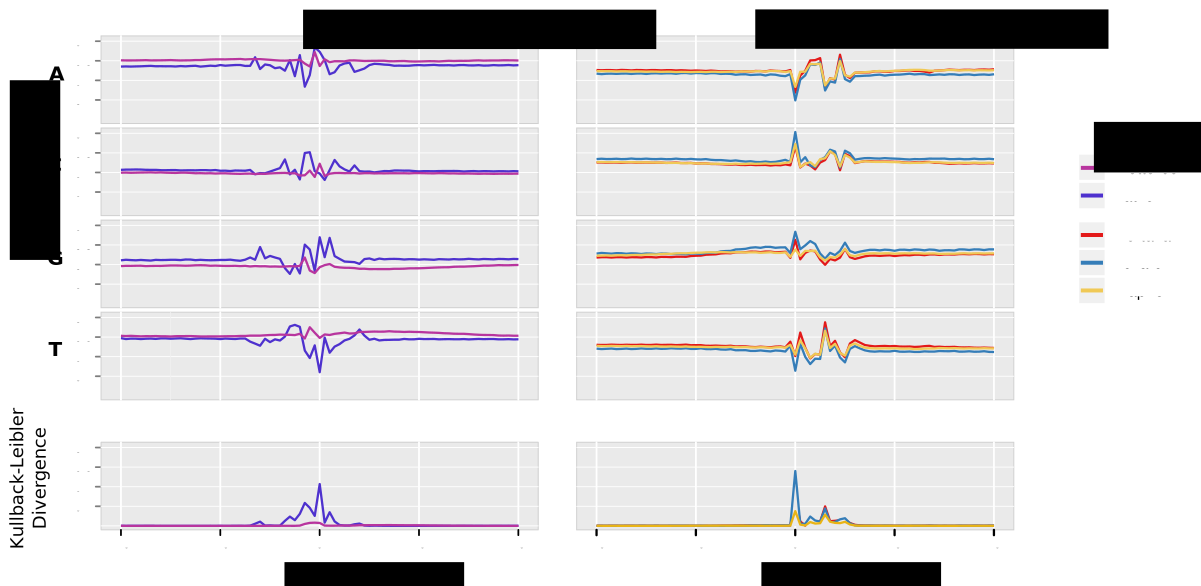
\includegraphics[width=0.8\textwidth]{fig/freqs.eps}}
\caption{Nucleotide frequencies are plotted relative to the start (labeled,
position 0) of each mapped read, respecting strand. The sequence is taken frmo
the genomic context surrounding the read, so that -40 to -1, for example, fall
outside the read sequence itself. The symmetrized Killback-Leibler divergence is
used to summarize the difference in nucleotide frequency compared to a fixed
estimate of background necleotide frequencies made by sampling many positions
nearby mapped reads.  Under the assumption that reads are sampled uniformly from
transcripts, each of the plots should be essentially flat.}
\label{fig:freqs}
\end{figure*}


Some work has been done to model and correct for these biases.  Li, et. al.,
\cite{Li2010} propose two models. The firsts is a Poisson linear model, in which
read counts across a transcript follow inhomogeneous Poisson process. The read
count at position $i$ within the transcript is Poisson distributed with
parameter $\lambda_i$, where, $\log(\lambda_i)$ is the sum of weights determined by the
nucleotide at each position surrounding the read start, in addition to a term
capturing the abundance of the transcript.

The second model is based on multiple additive regression trees, or MART
\cite{Friedman2003}.  In their tests, MART shows a moderate improvement over the
Poisson linear model. Both models are fit to a number of abundant test genes,
requiring existing gene annotations for the reference genome. 

Another model, proposed by Hansen, et. al., \cite{Hansen2010} directly estimates
the distribution of initial heptamers within reads, then estimates a presumed
background heptamer distribution by sampling from the end of reads. Read counts
are then adjusted by the ratio of the two. Specifying two distributions over
heptamers (i.e. foreground and background distributions) requires $2(4^7-1) =
32,766$ parameters, so while no gene annotations are needed to train such a
model, a significant number of reads are required.

Version 0.9.0 of Cufflinks \cite{Trapnell2010} also introduces a model to
correct for sequence bias. No description of their method is yet available, nor
is there any implementation of the model that can be run independently of
Cufflinks to facilitate testing, so we have withheld any comparison in our
tests.

Besides the direct influence of nucleotide composition on sequencing efficiency,
the ``uniqueness'' of a sequence within the genome affects how likely it is to
be mapped correctly, thus influencing quantification in a non-trivial way. Some
methods exist attempting to quantify uniqueness \cite{Koehler2010} and to take
it into account in the measure of transcript abundance \cite{Li2010b}
\cite{Lee2010}. Though we make no attempt to address this problem, any
probabilistic characterization of uniqueness or ``mapability'' could easily be
combined with the probabilistic characterization of sequence bias that we
described here.


\begin{figure}
\centerline{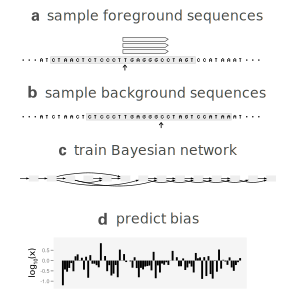
\includegraphics[width=0.35\textwidth]{fig/overview.eps}}
\caption{An overview of the approach taken: (a) foreground sequences are sampled
from the regions surrounding the starts of mapped reads, (b) background
sequences are sampled by randomly offsetting foreground positions, (c) a
Bayesian network is classifier is trained to descriminate between the set of
sampled foreground and background sequences, (d) and the classifier is evaluated
at each position within a locus, predicting bias.}
\label{fig:overview}
\end{figure}

\section{Methods}

\subsection{Principle}

We assume a simple model of an RNA-Seq experiment: the number of reads $x_i$
aligned to genomic position $i$ is an unbiased estimate of RNA abundance.
Furthermore, we assume reads may be treated as i.i.d. samples. That
is, if $N$ reads are generated, and $m_i$ is the event that a generated read
maps to position $i$,
$$ E[ x_i ] = N \Pr[ m_i ] $$


The experiment may be considered unbiased  with regards to sequence if having
observed the nucleotide sequence $s_i$ surrounding position $i$,
$$ E[ x_i | s_i ] = N \Pr[ m_i | s_i ] = N \Pr[ m_i ] = E[ x_i ] $$

From Bayes' rule,
$$ \Pr[ m_i | s_i ] = \frac{ \Pr[ s_i | m_i ] \Pr[ m_i ] }{ \Pr[ s_i ] } $$

This suggests a natural reweighing scheme. First, define the \emph{sequence
bias} $b_i$ at position $i$ as,
$$ b_i = \frac{ \Pr[ s_i ] } { \Pr[ s_i | m_i ] } $$

Now, if we reweight the read count at position $i$ by $b_i$, we
have,
\begin{align*}
E[ b_i x_i  | s_i ] &= b_i E[ x_i | s_i ] \\
&= N b_i \Pr[ m_i | s_i ] \\
&= N \frac{ \Pr[ m_i | s_i ] \Pr[ s_i ] }{ \Pr[ s_i | m_i ] } \\
&= N \Pr[ m_i ] \\
&= E[ x_i ]
\end{align*}
Thus the reweighted read counts are made to be unbiased.


To estimate the bias $b_i$, we must make estimates of the background sequence
probability $\Pr[s_i]$ and the foreground sequence probability $\Pr[ s_i | m_i
]$, the later being the probability of the sequence given a read being sampled
from its position. Any estimation of sequence probabilities presents a challenge
of finding a model that sufficiently complex to capture the common features of
the training data but avoids overfitting.

Towards that end, we propose training a Bayesian network classifier trained on
examples of foreground and background sequences. Though our goal is not
classification, by using the machinery of classification we can avoid a model
that is over-parametrized. Parameters that are not informative in
discriminating between foreground and background are not included in the model.
The Bayesian network can then used to evaluate sequence probability, and thus
bias at any genomic position.

This discussion so far ignores one complication. The RNA abundance that we wish to
estimate is not itself independent of of the nucleotide sequence. Notably,
exonic DNA is tends to be more GC-rich than intergenic DNA. If background
sequences are sampled uniformly from the genome we run the risk of incorrectly
adjusting for biological sequence bias, rather than technical sequence bias. To
avoid this, we propose using paired training data. Each foreground training
sequence is paired with a background sequence taken from nearby position that is
likely to have similar abundance and general nucleotide composition.
Alternatively, we could pair foreground samples with background samples from
within the same transcript, but we prefer to avoid dependence on existing gene
annotations as such a model would be less suitable for de-novo discovery or
annotation applications.

Hansen, et. al., \cite{Hansen2010} implicitly characterizes and corrects for
bias in the same manner proposed here. Their approach differs primarily in how
sequence probabilities are estimated. Li, et. al., \cite{Li2010} offers a
different perspective, taking advantage of gene annotations to train a model
that optimally explains variance in base level counts across transcripts.


\subsection{Estimation}

To estimate sequencing bias, we train a Bayesian network classifier in which
each node represents a position in the sequence, relative to the read start, and
edges encode dependency between positions. Bayesian networks have been
applied to recognize motifs in nucleotide sequences in the past, in particular
in modeling splice cites \cite{Cai2000} \cite{Chen2005} and transcription factor
binding sites \cite{Ben-Gal2005} \cite{Grau2006} \cite{Pudimat2005}. 

In our model, we do not rely on constraining the set of networks (e.g. to
trees), and instead approximate the NP-Hard problem of determining the optimal
network structure using a fast hill climbing algorithm. Furthermore, we
train our model \emph{discriminatively}; only parameters that are deemed
informative in discriminating between foreground and background sequences are
included in the model. We thus seek to train a model that reduces bias, without
including uninformative parameters that would only increase variance.


\subsubsection{Sampling}

To begin, we generate $n$ training examples, where $n = 200,000$ is typical, half of
which labeled as foreground, the other background. To do so, we sample the
positions of $n/2$ reads. Duplicate reads are ignored, to avoid overfitting to
any exceedingly highly expressed locus.  For each foreground position $i$
sampled, we then sample a background position by drawing a random offset $\delta
\sim \text{Normal}( 0, \sigma )$, where by default $\sigma = 50$ is chosen, and
taking $i' = \lceil i + \delta \rceil$. By using such a scheme we attempt to
mitigate the effects of biological sequence bias, sampling positions that are
more likely to be biologically similar.

This sampling procedure produces a set of $n$ genomic positions with
accompanying labels $T = \{ (i_1,x_1), (i_2,x_2), \dots, (i_n,x_n) \}$. The
label $x_k$ is binary, indicating classification as background ($x_{i_k} =
0$) or foreground ($x_{i_k} = 1$). We will denote the nucleotide sequence at
position $i_k$ as $s_{i_k}$.


\subsubsection{Training}

To determine the structure and parameters of the Bayesian network, we use a
hill-climbing approach similar to BNC algorithm \cite{Grossman2004}.
The network structure is determined by greedily optimizing the conditional
log-likelihood.
\begin{align*}
\ell &= \sum_{k=1}^{n} \log \Pr( x_{i_k} | s_{i_k} ) \\
&=
\sum_{k=1}^{n} \log \frac{ \Pr(s_{i_k} | x_{i_k}) \Pr( x_{i_k} ) }{
\sum_{x \in \{0,1\}} \Pr( s_{i_k} | x ) \Pr(x) } \\
%&= \sum_{k=1}^{n} \log \frac{ \Pr( s_{i_k} | x_{i_k} ) }
%{ \sum_{x \in \{0,1\}} \Pr( s_{i_k} | x ) }
\end{align*}

Where $\Pr(x)$ is flat (i.e.  $\Pr( x = 0 ) = \Pr( x = 1 ) =
0.5$) if we sample foreground and background positions equally.

As we will be estimating parameters and evaluating the likelihood on the same
set of samples, simply maximizing the likelihood would severely overfit the
training set. We thus penalize model complexity using the Akaike information
criterion with the second order sample size correction \cite{Hurvich1989}.
Where $m$ is the number of parameters needed to specify the model, we maximize,
$$ \ell' = \ell - m - \frac{(m + 1)(m + 2)}{n - m - 2} $$

At each step of the optimization procedure, every possible edge or position
addition, removal, or edge reversal that produces a valid network (i.e. does not
introduce a cycle) is evaluated, and the alteration that increases the score
$\ell'$ the most is kept.  This process is repeated until a local maxima is
found, in which no single alteration to the network will increase the score.

Given the network structure, the parameters are estimated directly from the
observed nucleotide frequencies. This choice of parameters maximizes the
likelihood of the model, but not necessarily the conditional likelihood. They
are equivalent asymptotically, thus, as per the BNC algorithm, we adopt this
approximation rather than  resorting to numerical methods which might render the
algorithm too slow to be practical.

The run time of the training procedure is further reduced in practice by imposing the
following two restrictions on the structure of the network,
\begin{enumerate}
\item The in-degree (i.e. number of parents) of any node must be less than some
number $p_{\text{max}}$.
\item $|j - i| \le d_{\text{max}}$ for all edges $(i,j)$ and some number $d_{\text{max}}$.
\end{enumerate}
The second of these encodes the assumption that distant nucleotides are
effectively independent.


\begin{comment}
\begin{figure*}
\begin{center}
\includegraphics[width=0.75\textwidth]{fig/structure2.pdf}
\end{center}
\caption{The network structure learned on the Trapnell data set, where 0 is the
read start. Dotted boxes represent positions not included in the model (i.e.
positions deemed uninformative).}
\label{fig:structure}
\end{figure*}
\end{comment}

Figure \ref{fig:structure} shows an example of the structure learned when this
procedure is applied to 200,000 reads from the Trapnell data set
\cite{Trapnell2010}. The structure learned is non-trivial, and
positions that uninformative are excluded automatically.


\section{Results}

Because we cannot observe directly the underlying RNA-abundance, our evaluation
strategy relies on testing two assumptions we make of an ideal, unbiased experiment.
\begin{enumerate}
\item Positional nucleotide frequencies (as in Figure \ref{fig:freqs}) measured
from reads within exons should not differ greatly from frequencies measured by
sampling uniformly within the same exons.
\item Read counts across exons should follow approximately a Poisson process.
\end{enumerate}

We applied our procedure (labeled ``BN'') as well as those of Li, et. al, and
Hansen, et. al., which are implemented in the R packages \texttt{mseq} and
\texttt{Genominator}, respectively. The procedures were applied to four publicly
available data sets \cite{Bullard2010} \cite{Mortazavi2008} \cite{Trapnell2010}
\cite{Wetterbom2010}, as well as an unpublished data set of our own (see, Table
\ref{tab:datasets}).

%% TODO
\begin{comment}
\begin{tablehere}
\begin{center}
\footnotesize{
\begin{tabular}{lllr}
\textbf{Experiment} & \textbf{Species} & \textbf{Platform} & \textbf{Read Length} \\ \hline
Wetterbom \cite{Wetterbom2010} & Chimpanzee & ABI & 33 \\
Katze (unpublished) & Macaque & ABI & 50 \\
Bullard \cite{Bullard2010} & Human & Illumina & 35 \\
Mortazavi \cite{Mortazavi2008} & Mouse & Illumina & 33 \\
Trapnell \cite{Trapnell2010} & Mouse & Illumina & 75
\end{tabular}
}
\end{center}
\caption{Data sets on which the methods are evaluated.}
\label{tab:datasets}
\end{tablehere}
\end{comment}


Testing was performed by cross-validation. Each method was trained on data taken
from chromosomes 1--8 of the genome from which the reads were mapped (including
chromosomes 2a and 2b in the Chimpanzee genome). For evaluation, we drew a set
long, highly expressed exons from the remaining chromosomes. In particular, for
each reference sequence, beginning with the set of exons annotated by Ensembl
release 60 \cite{Hubbard2009}, we removed any exons with known alternate splice
sites, then chose the top 1000 exons by read count, restricting ourselves those
at least 100nt long.

The differences in the methods being tested necessitated training procedures
unique to each.

Li recommends that their MART and GLM models be trained using the 100 most abundant
genes. We used 1000 exons from chromosomes 1--8, otherwise chosen in a manner
identical to that which was used to select the test exons.  Both the GLM and
MART model were trained using the default parameters.

Hansen recommends using all of the reads to estimate heptamer frequencies used by
their model. The training procedure works by simple tallying of frequencies and
is thus relatively fast. We choose to use all of the reads from chromosomes 1--8.
We evaluated three variations of this scheme. The first uses the default
parameters, evaluating 7-mer frequencies averaged over the first two positions
of the read (labeled ``Avg-7mer''). We also evaluated estimating 7-mer
frequencies over only the first position, as well as 4-mer frequencies over only
the first position. Though many variations of this scheme may be used, we found these
additional two to be particularly informative. The background frequencies in
each variation were were estimated from positions 18--23 within each read.

All data sets were mapped using Bowtie \cite{Langmead2009} against the latest
genome assemblies available from the UCSC Genome Browser \cite{Karolchik2008}
during preparation.



\subsection{Kullback-Leibler Divergence}

Plotting the nucleotide frequencies (Figure  \ref{fig:freqs}) we observe an
obvious bias. To quantify the non-uniformity observed in these plots, we use the
symmetrized Kullback-Leibler (KL) divergence \cite{Kullback1951}. Comparing only
nucleotide frequencies may miss dinucleotide or higher order bias. Thus, for a fair
comparison, we compute the KL divergence for $k$-mers, with $k \in \{ 1 \dots 6
\}$.

If $f_x$ is the background frequency of a $k$-mer $x$, and $f'_x$ the observed
frequency, the KL divergence is computed as,
$$D( f, f' ) = \sum_{x} \left( f_x \log( f_x / f'_x ) + f'_x \log( f'_x / f_x) \right)$$
Where the sum is over all $k$-mers. We compute the divergence at each
position relative to the read start, by tallying (overlapping) $k$-mer
frequencies at each position, weighted by the bias coefficient at that position,
and comparing to a background distribution. The background distribution is
estimated by averaging the $k$-mer frequencies at positions $-60 \dots -20$ and
$20 \dots 60$, where the observed bias was very low in each data set.  We further
take the precaution of ignoring any positions with more than 10,000 reads, to
avoid the measure being dominated by any small group of outliers. The only
qualitative effect this was seen to have was in the Katze data set, in which the
frequency plots are otherwise quite skewed.

The result of this this analysis is plotted in Figure
\ref{fig:kl} for the Trapnell data set. Similar plots for the other data sets are
provided in the supplement.

%% TODO
\begin{comment}
\begin{figurehere}
\begin{center}
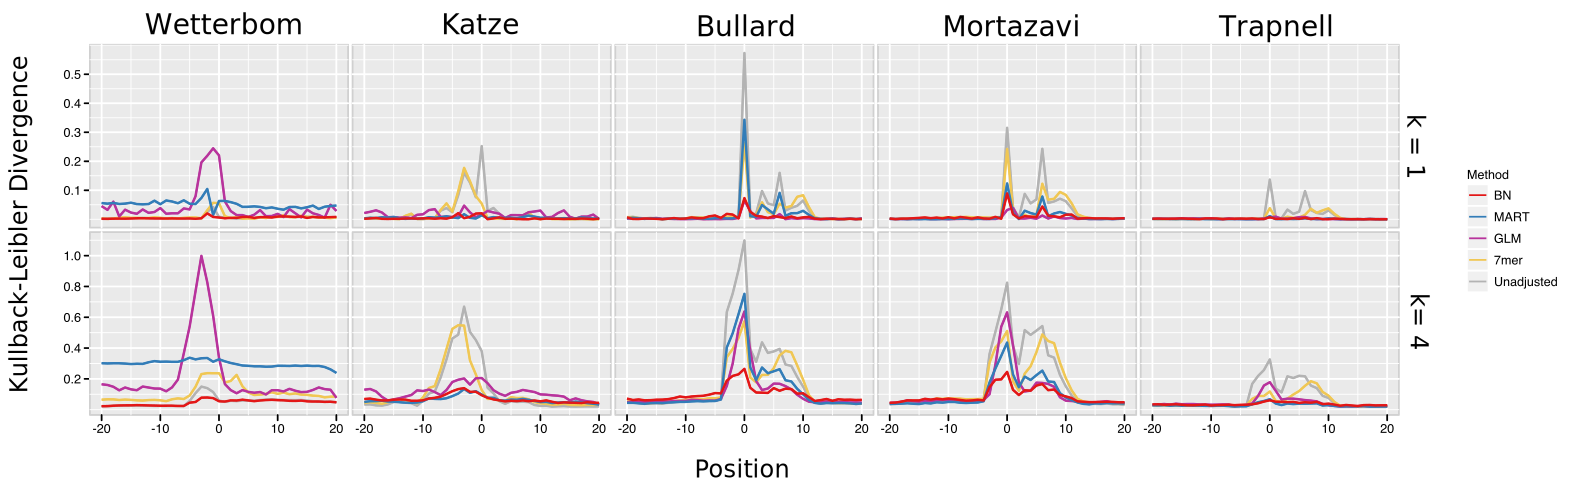
\includegraphics[width=0.5\textwidth]{fig/kl.pdf}
\end{center}
\caption{Plots of the KL divergence over overlapping $k$-mers in the Trapnell
experiment.}
\label{fig:kl}
\end{figurehere}
\end{comment}

To summarize these plots, we summed the divergence from position -20
through 20, for each of the methods, then normalized this number by dividing by
the summed divergence before adjustment. The results of this analysis are plotted in
Figure \ref{fig:kl-delta}.

%% TODO
\begin{comment}
\begin{figurehere}
\begin{center}
\includegraphics[width=0.35\textwidth]{fig/kl-delta.pdf}
\end{center}
\caption{Summed KL divergence, normalized by unadjusted divergence, so that a
number less than 1 indicates a decrease in divergence, or an increase in
uniformity.}
\label{fig:kl-delta}
\end{figurehere}
\end{comment}


\subsection{Poisson Regression}

In this comparison, we measure how well the counts conform to a Poisson process.
The assumption of positional read counts following a Poisson distribution has
been shown to be a poor fit \cite{Srivastava2010}, yet measuring the improvement in
fit derived from correcting for technical bias remains a principled and easily
interpreted criteria.

We perform maximum-likelihood fitting of two models. In the null model, the
Poisson rate is fixed for each exon. That is, for position $j$ within
gene $i$, the rate is,
$$ \lambda_{ij} = a_i $$
Where $a_i$ is the parameter being fit. For comparison, we then fit a model in
which the rate is proportional to the predicted bias coefficients.
$$ \lambda'_{ij} = a_i b_{ij} $$

If the null model has log-likelihood $L$ and the bias corrected model
$L'$, we measure the change in fit as,
$$ \log \left( \frac{ L_{i} } { L'_{i} } \right) $$
When the fit improves, this number is positive, and negative when it is
worsened. The values computed from our test are listed in Table \ref{tab:pois}.

\begin{comment}
\begin{tablehere}
\begin{center}
\tiny{
\begin{tabular}{lrrrrrr}
         &\textbf{Avg-7mer}&\textbf{7mer}&\textbf{4mer}&\textbf{GLM}&\textbf{MART}&\textbf{BN} \\
\textbf{Katze}            &  0.004  & 0.017  & 0.055 &0.166  &0.248&0.305 \\
\textbf{Wetterbom}        & -0.076  &-0.058  &-0.002 &0.240  &0.070&0.557 \\
\textbf{Bullard}          &  0.124  & 0.192  & 0.139 &0.285  &0.198&0.380 \\
\textbf{Mortazavi}        &  0.059  & 0.123  & 0.099 &0.284  &0.310&0.401 \\
\textbf{Trapnell}         &  0.094  & 0.163  & 0.104 &0.265  &0.332&0.349 \\
\end{tabular}
}
\end{center}
\caption{Change in fit, compared to the null model of uniform Poisson rate across exons.}
\label{tab:pois}
\end{tablehere}
\end{comment}

Computing one number to summarize the fit of the model ignores variance in the
likelihood from exon to exon. This number could be dominated by a few test
regions. Figure \ref{fig:pois} plots the distribution of the change in fit
across the 1000 test exons, revealing a similar, but more nuanced result.

%% TODO
\begin{comment}
\begin{figurehere}
\begin{center}
\includegraphics[width=0.4\textwidth]{fig/pois.pdf}
\end{center}
\caption{Plotted is the change in fit of each of the test exons. A
positive value indicates a better fit in the bias corrected model.}
\label{fig:pois}
\end{figurehere}
\end{comment}


\section{Discussion}

We have demonstrated that sequence bias can confound, sometimes severely,
quantification in RNA-Seq experiments, and we have introduced an effective
method to account for this bias without the need of existing gene annotations.

In our results, estimating initial 4-mer or 7-mer frequencies was not seen to be
as effective as the other models, even when data generated using random hexamer
priming was used. Given the large number of parameters needed to estimate 7-mer
frequencies, a likely explanation is that the model is overfit to the training
set. Though the training set consisted of at least 600,000 reads in
each experiment, it seems more reads, or a greater diversity of reads are needed
to produce an accurate estimate.

Our method generalizes this approach, attempting to overcome this problem by
using an estimation of sequence probability that is more robust to overfitting
and can account for bias beyond the initial heptamer. This approach is
competitive with that of Li, et. al., despite not requiring gene annotations.

Because we do not require annotations, CHiP-Seq, and other high-throughput
sequencing experiments, may also benefit from our model. In a preliminary
investigation, we found the sequence bias in one CHiP-Seq experiment
\cite{Cao2010} was less than that observed in any of the RNA-Seq data we
evaluated, however our method is still able effectively correct for the bias
that was observed (see, supplementary). Protocol differences, as we have seen,
can result in significant differences in observed nucleotide frequencies, so we
may not safely assert that bias in CHiP-Seq data is always low.  Given the weak
assumptions made by our model, our estimation of bias could easily be
incorporated into CHiP-Seq peak calling algorithms, and potentially improve
accuracy.

Our method can also very naturally capture dependency between nucleotides in the
sequence. This of particular importance when working with reads generated from
the AB SOLiD platform, in which the di-base, ``colorspace'' coding scheme is
used, encoding two adjacent nucleotides as a single color. A color bias at one
position will manifest itself as a nucleotide bias at two positions. Capturing
this effect requires a model that considers the dependency between nearby
positions. In our results, the MART model, as well as our own, perform
significantly better than the GLM model, illustrating this proposition.

RNA-Seq is most often used to compare levels of expression, and so a natural
concern is the consistency of the bias between samples. In the data we examined,
the bias appears to be largely, but not entirely consistent (see,
supplementary). Similarly, in Figure \ref{fig:freqs}, the three data sets
sequenced on the Illumina platform display similar patterns of nonuniformity,
yet differ in magnitude. Batch effects in RNA-Seq remain a legitimate concern,
that should be evaluated and corrected for.


\bibliographystyle{natbib}
\bibliography{seqbias-paper}

\end{document}



